	\documentclass[11pt, a4paper, spanish]{article}

\usepackage{alltt}

%%%%%%%%%% COMIENZO DEL PREAMBULO %%%%%%%%%%

%Info sobre este documento
\author{Mart\'n Cammi}
\title{Trabajo Pr\'actico de Algoritmos y Estucturas de datos III}

%\usepackage{infostyle}                                                  % provee un look & feel similar a un documento Word
\usepackage[top=2.5cm, bottom=2.5cm, left=2.5cm, right=2.5cm]{geometry}  % m\'argenes
\usepackage[ansinew]{inputenc}                                           % permite que los acentos del estilo \'a\'e\'i\'o\'u salgan joya
\usepackage[spanish, activeacute]{babel}                                 % idioma espaniol, acentos f\'aciles y deletreo de palabras
\usepackage{indentfirst}                                                 % permite indentar un parrafo a mano
\usepackage{caratula}                                                    % incluye caratula est\'andar
\usepackage{graphicx}                                                    % permite insertar gr\'aficos
\usepackage{color}                                                       % permite el uso de colores en el documento
\usepackage[pdfcreator={TexLive!, LaTeX2e con TeXnicCenter},
			pdfauthor={Grupo: "1"},
			pdftitle={Algoritmos III - Trabajo Pr\'actico 1},
			pdfsubject={Trabajo Pr\'actico 1},
			pdfkeywords={Torneo, Pizza, Goldbach},
			pdfstartview=FitH,            % Fits the width of the page to the window
			bookmarksnumbered,            % los bookmarks numerados se ven mejor...
			colorlinks,                   % links con bellos colores
			linkcolor=magenta]            % permite cambiar el color de los links
			{hyperref}                    % Permite jugar con algunas cosas que aparecer\'an en el PDF final

%RESTAURAR
\usepackage{algorithm}							% Permite tabular un codigo
\usepackage{algorithmic}
%\floatname{algorithm}{Algoritmo}
\renewcommand{\listalgorithmname}{Lista de algoritmos}
\renewcommand{\algorithmicrequire}{\textbf{Entrada:}}
\renewcommand{\algorithmicensure}{\textbf{Salida:}}
\renewcommand{\algorithmicend}{\textbf{fin}}
\renewcommand{\algorithmicif}{\textbf{si}}
\renewcommand{\algorithmicthen}{\textbf{entonces}}
\renewcommand{\algorithmicelse}{\textbf{si no}}
\renewcommand{\algorithmicelsif}{\algorithmicelse,\ \algorithmicif}
\renewcommand{\algorithmicendif}{\algorithmicend\ \algorithmicif}
\renewcommand{\algorithmicfor}{\textbf{para}}
\renewcommand{\algorithmicforall}{\textbf{para todo}}
\renewcommand{\algorithmicdo}{\textbf{hacer}}
\renewcommand{\algorithmicendfor}{\algorithmicend\ \algorithmicfor}
\renewcommand{\algorithmicwhile}{\textbf{mientras}}
\renewcommand{\algorithmicendwhile}{\algorithmicend\ \algorithmicwhile}
\renewcommand{\algorithmicloop}{\textbf{repetir}}
\renewcommand{\algorithmicendloop}{\algorithmicend\ \algorithmicloop}
\renewcommand{\algorithmicrepeat}{\textbf{repetir}}
\renewcommand{\algorithmicuntil}{\textbf{hasta que}}
\renewcommand{\algorithmicprint}{\textbf{imprimir}} 
\renewcommand{\algorithmicreturn}{\textbf{devolver}} 
\renewcommand{\algorithmictrue}{\textbf{cierto }} 
\renewcommand{\algorithmicfalse}{\textbf{falso }} 
 % mi archivo de traducci\'on			

%\selectlanguage{spanish}

%\selectlanguage{spanish}
\linespread{1.3}                    % interlineado equivalente al 1.5 l\'ineas de Word...
\pagestyle{myheadings}              %encabezado personalizable con \markboth{}{}
\markboth{}{Algoritmos III  - Trabajo Pr\'actico 1 - Cammi, Garbi, Kretschmayer}
\headsep = 30pt                     % separaci\'on entre encabezado y comienzo del p\'arrafo

%\addtolength{\oddsidemargin}{-2cm}	% configuracion IDEAL!!!
%\addtolength{\textwidth}{4cm}
%\addtolength{\textheight}{2cm}

% macro 'todo' para To-Do's
\def\todo#1{\textcolor{red}{#1}}

% Macro 'borde' para un texto con borde
\newsavebox{\fmbox}
\newenvironment{borde}[1]
{\begin{lrbox}{\fmbox}\begin{minipage}{#1}}
{\end{minipage}\end{lrbox}\fbox{\usebox{\fmbox}}\\[10pt]}

%%%%%%%%%% FIN DEL PREAMBULO %%%%%%%%%%

\begin{document}

\materia{Algoritmos y Estucturas de datos III}
\submateria{Segundo Cuatrimestre de 2011}
\titulo{Trabajo Pr\'actico 1}
\subtitulo{Problema1: Torneo. \ \ \ \ \ \ \ \ \ \ \ \ \ \ \ \ \ \ \ \ \ \ \ \ \ \ \ \ \ \ \ \ \ \ \  Problema2: Pizza entre amigos. \ \ \ \ \ \ \ \ \ \ \ \ \ \ \ \ \ \ Problema3: Conjetura de Goldbach.}
\grupo{Grupo: `1'}
\integrante{Cammi, Mart\'in}{676/02}{martincammi@gmail.com}
\integrante{Garbi, Sebasti\'an}{179/05}{garbyseba@gmail.com}
\integrante{Kretschmayer, Daniel}{310/99}{daniak@gmail.com}

\maketitle

\thispagestyle{empty}

\tableofcontents

\newpage


\textbf{Ejecuci\'on del TP}
\label{sec:ejecucion}

	\subsection{Lenguaje utilizado}
		
		El lenguaje utilizado para el trabajo pr\'actico ha sido \emph{Java}, compilando con la versi\'on 1.5 de la Virtual Machine.
		
		El trabajo se acompa\~{n}a con los fuentes de la soluci\'on que puede importarse en IDE de Eclipse o ejecutarse desde l\'inea de comandos.

	\subsection{Como ejecutar el TP}
	
	\textbf{\underline{Desde l\'inea de comandos}}
	\begin{itemize}
			\item{Posicionarse en el directorio Algo3Tp1}
			\item{Copiar all\'i el archivo de entrada para el problema i, por ejemplo Ej1.in}
			\item{Ejecutar el comando: \emph{java -cp ./bin problema1.Ej1}}
	\end{itemize}
	Esto generar\'a el archivo Ej1.out con la soluci\'on en el mismo directorio Algo3Tp1.

	\textbf{\underline{Desde el Eclipse}}
	
	Primero importaremos el proyecto:	
	
	\begin{itemize}
			\item{Seleccionar File $\Rightarrow$ Import.}
			\item{Seleccionar General $\Rightarrow$ Existing Projects into Workspace $\Rightarrow$ Next.}
			\item{Seleccionar el directorio llamado Algo3Tp1.}
			\item{Finish.}
	\end{itemize}
	
	Desde la vista de \textbf{Package Explorer} bajo el paquete \textbf{src} aparecer\'an tres paquetes m�s y dentro de cada uno de ellos los siguientes archivos de java:\\

	\begin{center}
		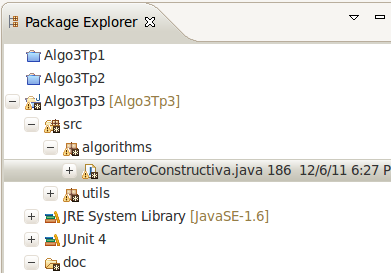
\includegraphics[scale=0.65]{others/packageExplorer.png}\\
	\end{center}

\newpage

	Para ejecutar un problema:

	\begin{itemize}
			\item{Posicionarse en el directorio Algo3Tp1}
			\item{Copiar en el directorio Algo3Tp1 el archivo de entrada para el problema i, por ejemplo Ej1.in}
			\item{Con bot\'on derecho Run As $\Rightarrow$ Java Application. Se ejecutar\'a el problema seleccionado.}
	\end{itemize}
	Esto generar\'a el archivo Ej1.out con la soluci\'on en el mismo directorio Algo3Tp1.

\newpage

% Conviene poner las secciones como diferentes archivos,
% sobre todo cuando se trabaja en equipo.
% Es m\'as f\'acil para sincronizar mediante control de versiones.
%\input{Introducci\'on}

% Problema1
\section{Problema1: Torneo}
\label{sec:problema3}
	\subsection{Introducci\'on}
	
	  Debemos organizar un torneo que involucre a n competidores. Cada competidor debe jugar exactamente una vez con cada uno de sus oponentes. Adem\'as, cada competidor debe jugar un partido por d\'ia con la sola posible excepci\'on de un d\'ia en el cual no juegue. \\
	  
		Para ello, implentaremos un algoritmo que utilice la t\'ecnica de divide y vencer\'as. Si la cantidad de competidores es potencia de $2$ o es par, el torneo debe terminar en $n-1$ d\'ias. En cambio si n es impar, el torneo debe terminar en $n$ d\'ias.

	\subsection{Explicaci\'on de la soluci\'on}
	
	Para que un torneo se pueda armar, el n\'umero de competidores debe ser mayor o igual a $2$. En cambio, en caso de venir menor cantidad de jugadores, el algoritmo no crear\'a el torneo, ya que no tiene sentido realizarlo. \\
	
	Para resolver el problema, utilizamos una matriz como estructura de almacenamiento, donde iremos guardando la tabla de los partidos entre cada jugador, y en que dias \'estos competir\'an. La matriz tiene como filas, la cantidad de jugadores del torneo, y como columnas la cantidad de dias que demandar\'a este. En ambos casos, no utilizamos el \'indice 0, solo para facilitar la legibilidad del algoritmo.\\
	
	En cada llamada recursiva, el torneo se divide de a mitades, pero nosotros llamamos a recursi\'on solo con la primera de ellas, y luego realizamos la etapa de combinaci\'on, que termina calculando las competiciones para la otra mitad de jugadores.\\
	
	Cuando la cantidad de competidores totales (o en cualquier llamada recursiva) es impar, lo que realiza el algoritmo es la de agregar un jugador "`ficticio"', y se genera el torneo como si este fuese uno real. Para distinguirlo, utilizamos una funci\'on que pone a ese jugador como el jugador $0$. Luego, es la etapa de combinaci\'on la encargada de asignarle a ese jugador su oponente para ese d\'ia, o caso contrario, implicar\'a que el jugador tiene fecha libre ese d\'ia, por lo que la matriz final quedar\'a en $0$.\\
	
	El caso base del algoritmo es cuando quedan $2$ jugadores, que los hace competir en el d\'ia 1 entre si. 

\newpage
	
\subsection{Pseudo-c\'odigo}
	
\begin{algorithm}
\caption{Torneo}
\label{alg1}
\begin{algorithmic}

	%Para mas referencia ver http://en.wikibooks.org/wiki/LaTeX/Algorithms_and_Pseudocode
	\STATE	crearTorneo(cantJugadores)
	\IF {cantJugadores == 2}
		\STATE	fixturePartidos[1][1] = 2;							
		\STATE	fixturePartidos [2][1] = 1;	  					
	\ELSE
			\IF {(cantJugadores mod 2)!=0}  \STATE	//cantidad jugadores impar
				\STATE	torneo(cantJugadores+1);      		
				
				\STATE	colocarJugadorFicticio(cantJugadores);  
			\ELSE   \STATE	//si cantJugadores es par
				\STATE	mitadJugadores = cantJugadores / 2; 
				\STATE	torneo(mitadJugadores);  // primero el cuadrante sup. izq.  
				
				\STATE	boolean esPar = (mitadJugadores mod 2) ==0;
				\STATE	cuadranteInferiorIzquierdo(mitadJugadores, cantJugadores, esPar);
				\STATE	cuadranteInferiorDerecho(mitadJugadores, cantJugadores, esPar);
				\STATE	cuadranteSuperiorDerecho(mitadJugadores, cantJugadores, esPar);
			\ENDIF
	 \ENDIF
	 
\end{algorithmic}
\end{algorithm}	

\subsection{Modelo Elegido}
	Para calcular la complejidad de este algoritmo utilizaremos el modelo $Uniforme$, ya que la cantidad de jugadores de un torneo no es significativamente grande, por lo que la cantidad de bits para representar cualquier jugador no deber\'ia ser grande, por lo que consideramos que las operaciones para sumar y restar es constante y podemos asumirla en $O(1)$

\newpage
	
\subsection{Complejidad}
	
\begin{algorithmic}
	
	 \STATE	cuadranteInferiorIzquierdo(mitadJugadores, cantJugadores, esPar)
	 \IF {esPar}
			\FOR {cada jugador entre mitadJugadores+1 y cantJugadores}
				\FOR {cada dia entre 1 y mitadJugadores-1}
						\STATE	fixturePartidos[jugador][dia] = fixturePartidos[jugador-mitadJugadores][dia] + mitadJugadores;
				\ENDFOR
			\ENDFOR
		\ELSE
			\FOR {cada jugador entre mitadJugadores + 1 y cantJugadores} 
				\FOR {cada dia entre 1 y mitadJugadores}
					\IF {fixturePartidos[jugador - mitadJugadores][dia] == 0} 
						\STATE	fixturePartidos[jugador][dia]=0;
					\ELSE
						\STATE	fixturePartidos[jugador][dia]= fixturePartidos[jugador-mitadJugadores][dia] + mitadJugadores;
					\ENDIF
				\ENDFOR
			\ENDFOR
			\STATE	sacarJugadorFicticio(mitadJugadores);
		\ENDIF
		
		\STATE	colocarJugadorFicticio(cantJugadores)
		\FOR {cada jugador entre 1 y cantJugadores}  
			\FOR {cada dia entre 1 y cantJugadores}
				\IF {fixturePartidos[jugador][dia] == cantJugadores+1}
					\STATE	fixturePartidos[jugador][dia]= 0;
				\ENDIF
			\ENDFOR
		\ENDFOR
		
		\STATE	sacarJugadorFicticio(mitadJugadores)
		\FOR {cada jugador entre 1 y mitadJugadores} 
			\FOR {cada dia entre 1 y mitadJugadores}
				\IF {fixturePartidos[jugador][dia] == 0} 
					\STATE	fixturePartidos[jugador][dia] = jugador + mitadJugadores; 
	 				\STATE	fixturePartidos[jugador+mitadJugadores][dia] = jugador;
				\ENDIF
			\ENDFOR
		\ENDFOR
	
			
\end{algorithmic}	

\newpage

	El costo del algoritmo es el orden que tarda la combinaci\'on m\'as el costo de dividir.
	
	Si analizamos la combinaci\'on, veamos primero cual es el orden de cuadranteInferiorIzquierdo. Este recorre $n/2$ jugadores, y para cada uno de ellos, chequea $n/2$ dias para realizar los cruces en el torneo. El tiempo que se demora para hacer esta iteraci\'on es de $O((n/2)^{2}$. Adem\'as, luego de crear los partidos entre estos competidores, si fue llamado con un n\'umero impar, debe sacar los jugadores ficticios, que nuevamente recoore n/2 jugadores, $n/2$ d\'ias. Por lo que, en el peor caso (si n es impar), el algoritmo tiene costo $O(n^{2}/2)$.\\  
	
	El an\'alisis para cuadranteInferiorDerecho, y cuadranteSuperiorDerecho es an\'aalogo el de cuadranteInferiorIzquierdo, pero no debe colocar al jugador ficticio, por lo que el orden de cada uno es de $O((n/2)^{2})$.

	Por lo que, si sumamos los 3 cuadrantes, m\'as colocar el jugador ficticio, el tiempo que se demora es $O(n^{2})$. Notes\'e tambi\'en, cuando la llamada recursiva tiene cantidad de jugadores impar, debe sacar al jugador ficticio que se agrego previamente, y el orden de este algoritmo tambi\'en es de $O(n^{2})$.\\
	
	Como realizamos siempre la subdivisi\'on en 2 veces, la cantidad de subdivisiones que realiza el algoritmo es $log(n)$ veces.\\
	
	Por lo tanto, el algoritmo se demora en total, $O(n^{2} * log(n))$.\\
	
	Ahora debemos calcular el algoritmo en funci\'on del tama\~{n}o de entrada.\\
	
	\begin{center}
	$T = \log n$\\
	\end{center}
	
	\begin{center}
	ya que para representar un n\'umero n, se necesitan $\log n$ bits, entonces
	\end{center}

	\begin{center}
	$n = 2^{T}$.
	\end{center}

	\begin{center}
	La complejidad del algoritmo en funci\'on del tama\~{n}o de entrada es entonces de
	\end{center}

	\begin{center}
	 $O(2^{T} \cdot log 2^{T})$
	\end{center}

	\begin{center}
	Que equivale a:
	\end{center}

	\begin{center}
	$O(2^{T} \cdot T)$
	\end{center}



\newpage

\subsection{Tests}
	
	Si estudiamos previamente como est\'a formado el algoritmo, podemos preveer que este se comportar\'a mejor con n\'umeros que son potencia de 2, ya que no debe colocar ni sacar jugadores ficticios. Por otro lado, con que m\'as veces realice esta operaci\'on de agregar y sacar jugadores que no forman parte del torneo, el algoritmo a priori, deber\'ia ser m\'as costoso.
	 Realizaremos distintas mediciones, para conocer si estas previsiones son reales o no. Trataremos de realizar torneos con 3 tipos de datos de entrada.\\
	 
	 \textbf{Tipo 1)} Usaremos n\'umeros potencia de 2, para ver si efectivamente, el algoritmo presenta un mejor caso para este tipo de torneos.\\

	 \textbf{Tipo 2)} Realizaremos torneos con cantidad de jugadores impares, donde este n\'mero sea igual a un n\'mero potencia de $2$ sumado $1$. Con este tipo de valores ( y m\'as para n\'umeros grandes) trataremos de corroborar si efectivamente es un peor caso o no.\\

	 \textbf{Tipo 3)} Por \'ultimo, haremos mediciones con n\'umeros que no pertenezcan a los primeros 2 tipos, para ver como se comporta el algoritmo, y si estamos en presencia de alg\'un mejor o peor caso. 
	
\subsection{Gr\'aficos}

	\begin{center}
		\includegraphics[scale=0.65]{p1/p1ComparativoEscalaNormal.png}\\
	\end{center}
	\begin{center}
		\includegraphics[scale=0.65]{p1/p1ComparativoEscalaLogaritmica.png}\\
	\end{center}
	\begin{center}
		\includegraphics[scale=0.65]{p1/p1MejorEscalaNormal.png}\\
	\end{center}
	\begin{center}
		\includegraphics[scale=0.65]{p1/p1MejorEscalaLogaritmica.png}\\
	\end{center}
	\begin{center}
		\includegraphics[scale=0.65]{p1/p1PeorEscalaNormal.png}\\
	\end{center}
	\begin{center}
		\includegraphics[scale=0.65]{p1/p1PeorEscalaLogaritmica.png}\\
	\end{center}

\subsection{Conclusiones}

	Hemos podido notar, que el algoritmo se comporta de acuerdo a lo esperado. Los mejores casos del algoritmo es cuando la cantidad de jugadores es potencia de $2$, y los peores son cuando la cantidad de jugadores es de la forma $(2^{i}+1)$, con $i$ cualquier n\'umero entero mayor a $1$. Por otro lado, los n\'umeros restantes se comportan de acuerdo a la cantidad de veces que deban realizar estas operaciones de agregar y sacar ficticios, pero no son ni los mejores, ni los peores casos.
\newpage

% Problema2
\section{Problema2: Pizza entre amigos}
\label{sec:problema2}
	\subsection{Introducci\'on}
	Se quiere pedir una pizza extra gigante para un grupo de amigos. Cada uno de los amigos tiene su preferencia de elementos que quiere que est\'en en la pizza y elementos que preferir\'ia que no est\'en.
	Como quiz\'as no sea posible satisfacer todas las preferencias de cada uno de los amigos, se pretende buscar una soluci\'on donde al menos una de las preferencias de cada amigo sea satisfecha �, de no encontrarse una soluci\'on, responder que no es posible.
	\subsection{Explicaci\'on de la soluci\'on}
	Antes de explicar la soluci\'on elegida, comentaremos algunas decisiones tomadas ad hoc:
	\begin{itemize}
		\item En la entrada puede llegar a venir en las preferencias de alguno de los comensales un ingrediente repetido. Se descartaran las apariciones repetidas de ese ingrediete en caso que la decisi\'on tomada sobre el mismo sea la misma. Por ejemplo las instancia +A+B+A ser� equivalente a la instancia +A+B.
		Si alguna de las repeticiones tiene la decisi\'on contraria por ejemplo en el caso de +A+B-A, entonces asumiremos que este comensal est\'a satisfecho ya que cualquier decisi\'on tomada sobre el ingrediente en cuesti\'on lo satisfacer\'a.
		\item Otro caso ad hoc es cuando en la entrada viene una linea vacia (solo ';'), en este caso asumiremos que no existe una pizza que satisfaga al menos una preferencia de este comensal ya que este no tiene preferencias.
	\end{itemize}

Fuera de estos casos, asumimos que todos los comensales tienen al menos una preferencia para la pizza.\\

	La idea del algoritmo es, usando backtracking, ir recorriendo un arbol de decisi\'on donde la altura esta dada por la cantidad de ingredientes posibles + $1$ y cada nivel $i$ del arbol se corresponde al iesimo ingrediente cuyos subarboles son de las decisiones de poner o no ese ingrediente en la Pizza.\\
	
En las hojas de este \'arbol estan todas las posibles combinaciones de pizza, si ya se revisaron todas las posibles combinaciones y ninguna cumpli\'o entonces no hay soluci\'on para esas preferencias.
	
En cada iteraci\'on del algoritmo se van marcando los comensales que fueron satisfechos con la desici\'on tomada sobre el ingrediente actual, cuando se llega al �ltimo ingrediente si todos los comensales estan marcados se devuelve esa pizza, si no se desmarcan y se prueba por otra rama del arbol y se repite el proceso.\\

\textbf{Poda1:} Se puede ir chequeando a medida que se va armando la soluci\'on parcial si ya todos los comensales fueron marcados, si pas\'o esto se puede terminar antes ya que la soluci\'on parcial es la misma que no poner el resto de los ingredientes.\\

\textbf{Poda2:} En cada iteraci\'on se chequean solo los comensales que no hayan sido marcados ya en la soluci\'on parcial actual, ya que los demas est\'an satisfechos y seguir\'an est\'andolo cualquiera sea la desici\'on que se tome sobre el resto de la pizza.\\

\textbf{Poda3:} Antes de armar el \'arbol se revisan las preferencias de cada uno de los comensales para ver cuales son los ingredientes que realmente importan ya que si nadie tiene preferencia (ya sea por que vaya o no en la pizza) sobre alg�n ingrediente obviaremos revisarlo.\\

\textbf{Poda4:} Como estamos recorriendo el \'arbol de decisi\'on desde la primera hasta la �ltima letra (ingrediente) en orden, podemos saber cuando un comensal no va a poder ser satisfecho con la soluci\'on parcial actual comparando el ingrediente actual con el "Mayor" en los que tiene una preferencia el comensal.\\

   \textbf{Poda5:} En el caso de estar evaluando la rama true de un ingrediente y no sacar ning\'un comensal, esto quiere decir que de los que quedan, nadie tiene decisi\'on sobre ese ingrediente o bien los que la tienen prefieren que no vaya. Si contin\'uo evaluando esta rama y llego a una soluci\'on, tambi\'en llegar\'e no poniendolo. En cambio si no llego a una soluci\'on y nadie ten\'ia preferencia que no vaya, tampoco lo har\'e en la rama false. En cuyo caso me basta con evaluar s\'olo la rama false y me evito hacer dos veces el subarbol que queda con los proximos ingredientes.\\

\textbf{Tip:} Vamos marcando junto con los comensales que fueron satisfechos que ingrediente los satisfiso para que, si hay que retroceder en el \'arbol, se desmarquen solo esos y se contin�e probando con otra soluci\'on.\\

\newpage
	\subsection{Pseudo-c\'odigo}
	\begin{algorithm}			% enter the algorithm environment
	\caption{EncontrarPizza}		% give the algorithm a caption
	\label{alg1}  				% Para mas referencia ver http://en.wikibooks.org/wiki/LaTeX/Algorithms_and_Pseudocode
	\begin{algorithmic}
	
	\STATE i $\gets$ PrimerIngredienteImportante
	\STATE pizza $\gets$ pizzaVacia
	\STATE ponerEnLaPizza $\gets$ \TRUE
	\IF{ backtrack(i, ponerEnLaPizza) }
		\RETURN pizza
	\ELSE
		\IF{ backtrack(i, !ponerEnLaPizza)}
			\RETURN pizza
		\ELSE
			\RETURN sin soluci\'on
		\ENDIF
	\ENDIF
	\end{algorithmic}
	\end{algorithm}
	\begin{algorithmic}
	\STATE backtrack(i, ponerEnLaPizza)
	\IF{ponerEnLaPizza == \TRUE}
		\STATE poner i en la pizza
	\ENDIF
	\STATE marcar comensales satisfechos 
	\IF {no hay mas comensales insatisfechos} 
		\RETURN \TRUE
	\ELSE
		\IF{quedan ingredientes sin mirar} 
			\STATE i $\gets$ siguienteIngrediente 
			\IF{ backtrack(i, ponerEnLaPizza)}
				\RETURN \TRUE
			\ELSE
				\IF{backtrack(i,\TRUE)}
					\RETURN \TRUE
				\ELSE
					\STATE i $\gets$ anteriorIngrediente
				\ENDIF
			\ENDIF
		\ENDIF
		\STATE desmarcar comensales satisfechos
		\IF{ponerEnLaPizza == \TRUE}
			\STATE sacar i de la pizza
		\ENDIF
		\RETURN \FALSE
	\ENDIF
	\end{algorithmic}	
	\subsection{Modelo Elegido}
	Para calcular la complejidad de este algoritmo utilizaremos el modelo $Uniforme$, ya que por m\'as que la cantidad de datos de la entrada crezca, las operaciones sobre cada uno de ellos es constante y podemos asumirla en $O(1).$
	\subsection{Complejidad}

	\noindent{Siendo:}\\
	$n$ = Cantidad de Ingredientes\\
	$m$ = Cantidad de Comezales\\

	\noindent{Las siguientes acciones toman:}
	\noindent{$O(1)$ Preguntar si un comensal prefiere un ingrediente}\\
	$O(1)$ Preguntar si quedan comensales insatisfechos\\
	$O(n)$ Armar la soluci\'on\\
	$O(1)$ Mover un comensal de una lista a otra\\
	   (ya sea vaciando una lista de principio a fin o removiendo del iterador)\\
	
	En peor caso el algoritmo recorre todos los nodos del arbol y estos son $2^{n+1} - 1$
	o sea $O(2^{n})$.
	Por cada vez que recorre un nodo itera sobre todos los comensales insatisfechos restantes
	En peor caso esto es $O(m)$.
	
	Esto deja el algoritmo en una complejidad teorica de $O(2^{n}*m)$.\\
	Considerando que n es acotado por la cantidad de letras en el alfabeto ingles (26) el algoritmo queda dependiendo solo de m o sea $O(m)$.\\
	
	Para describir la complejidad en funci\'on el tama�o de entrada debemos considerar que cada comensal puede llegar a tener hasta $26$ preferencias, estos son $52$ caracteres por comensal\\

	Definimos el tama�o de entrada como:

	\begin{center}	
	$T = log(m*n*2)$\\
	\end{center}

	Sabiendo que n es acotado tomamos:
	\begin{center}	
	$T = log(m)$\\
	\end{center}

	Como la complejidad del algoritmo es $O(m)$ despejamos $n$ en funcion de $T$:
	\begin{center}	
	$m = 2^{T}$\\
	\end{center}	

	\subsection{Tests}
	\textbf{Tipo1:} Un estudio poco profundo nos dir\'ia que los peores casos son aquellos que tiene todas las permutaciones. A estos los llamaremos de $Tipo 1$\\
	Ej.
	\begin{verbatim}
	3
	+A+B+C;
	+A+B-C;
	+A-B+C;
	+A-B-C;
	-A+B+C;
	-A+B-C;
	-A-B+C;
	-A-B-C;
	.
	\end{verbatim}

	\textbf{Tipo2:}	Investigando un poco m\'as el algoritmo pudimos observar que los peores casos para cada tama�o de entrada ocurrir\'an cuando tenga que evaluar cada ingrediente en la mayoria de los comensales.\\

	Sabiendo que el algoritmo primero intenta poner el ingrediente y luego, en caso que no haya soluci\'on prueba no poniendolo lo obligamos a hacer el mayor n\'umero de operaciones por la rama true.\\

	Tambien tenemos que procurar que no termine hasta haber revisado el \'ultimo ingrediente as\'i que ponemos algun comensal que tenga una preferencia contraria. Si ese comensal tiene m\'as de una preferencia entonces se podr\'ia satisfacer evitando que se revisen m\'as ingredientes as\'i que no le ponemos m\'as.
	Los peores casos ser\'ian de la forma:
	\begin{verbatim}
	3
	+A+B+C;
	+A+B+C;
	...
	+A+B-C;
	+A-B;
	-A;
	.
	\end{verbatim}

\newpage

	\textbf{Tipo3:} Finalmente observamos que los casos de $Tipo 2$ descartaban la decisi\'on de poner un ingrediente casi de inmediato as\'i que intentamos buscando un caso peor a�n y nos pusimos la meta de no descartar letras con el podado y ademas que eval\'ue la mayor cantidad posible de comensales en cada nodo. La soluci\'on fue la siguiente:
	\begin{verbatim}
	26
	+A+B+C+D+E+F+G+H+I+J+K+L+M+N+O+P+Q+R+S+T+U+V+W+X+Y+Z;
	+Z;
	+Z;
	 ...
	+Z;
	-Z;
	.
	\end{verbatim}	

\newpage

	\subsection{Gr\'aficos}
	%grafico tipo 1
	\begin{center}
		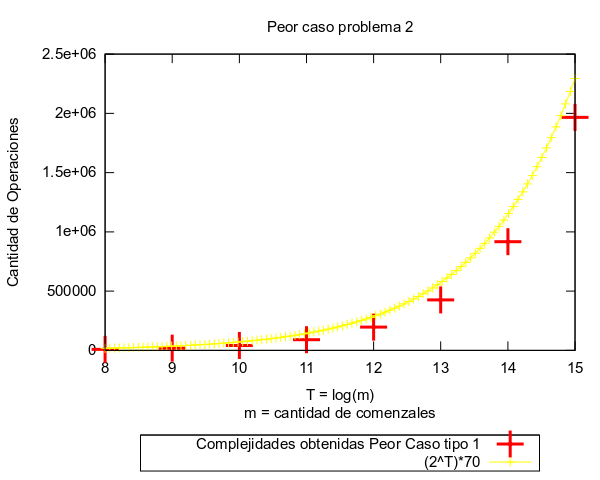
\includegraphics[scale=0.60]{p2/Problema2GraficoTipo1.png}
	\end{center}

En el gr\'afico aparecen marcadas con X rojas los peores casos para tama�os de entradas desde 8 bits a 15 bits. La funci\'on te\'orica aumentada 70 veces logra acotar bastante bien la cantidad de operaciones del algoritmo. El problema es exponencial con respecto al tama\~{n}o de la entrada. Los gr\'aficos siguientes muestran similares conclusiones variando la constante mutiplicativa.\\

	%grafico tipo 2
	\begin{center}
		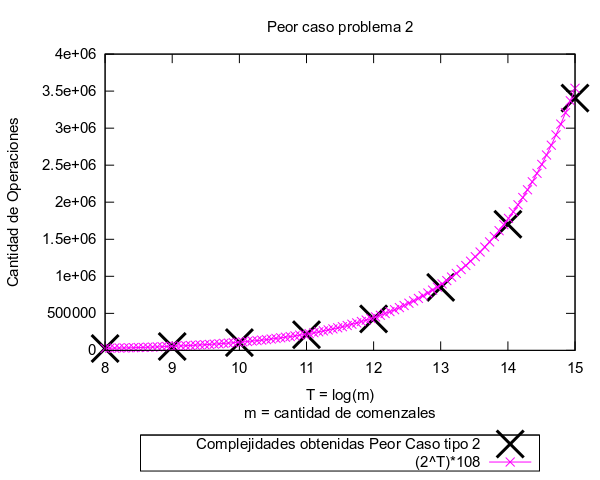
\includegraphics[scale=0.60]{p2/Problema2GraficoTipo2.png}\\
	\end{center}
\newpage

	%grafico tipo 3
	\begin{center}
		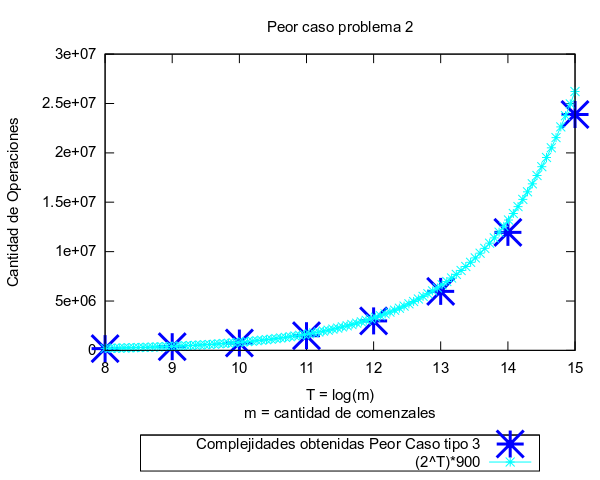
\includegraphics[scale=0.65]{p2/Problema2GraficoTipo3.png}\\
	\end{center}

	En general, los tres gr\'aficos muestran los peores casos en donde las mediciones obtenidas concuerdan con la complejidad teorica que habiamos calculado. Se puede observar tambi\'en  que las constantes utilizadas para comparar las mediciones con la funci\'on son mucho menores de lo que habiamos calculado en un primer momento como $2^{26}$.
	Esto puede deberse a que si un comensal no es marcado en una decisi\'on sobre un ingrediente, puede ser marcado en la contraria achicando el conjunto de comensales a evaluar.\\

	\begin{center}
		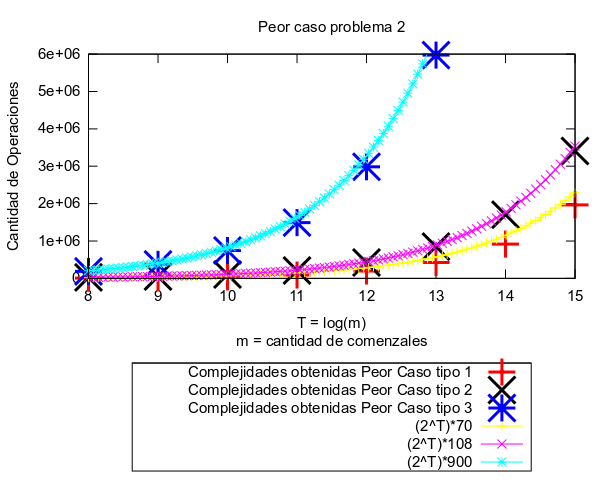
\includegraphics[scale=0.65]{p2/Problema2GraficoComparacionDeLos3Tipos.png}
	\end{center}

	En este \'ultimo gr\'afico se puede comparar las mediciones de los tres tipos de casos juntas. Se puede ver que efectivamente el caso $Tipo 3$ es el peor de todos ya que el primer comensal hace participar todos los ingredientes y nunca se filtran los comensales hasta llegar al �ltimo ingrediente.

  \subsection{Conclusiones}
    Luego de estudiar bastante el problema, y tratando de utilizar las nuevas t\'ecnicas aprendidas hasta el momento, llegamos a la conclusi\'on que atacar el problema con \emph{Backtracking} era lo m\'as l\'ogico.\\

    Pensamos en un algoritmo \emph{Goloso}, pero cualquier decisi\'on arbitraria que tom\'aramos sobre alg\'un ingrediente en particular pod\'ia ser facilmente rota poni\'endo un participante con la preferencia contraria unicamente.\\

    Con \emph{Divide and Conquer} podr\'iamos haber dividido la cantidad de comensales, pero podr\'iamos haber llegado a subsoluciones incompatibles al momento del merge, mientras que una soluci\'on geneal era posible.\\

    Con Programaci�n Din\'amica ten\'iamos un problema parecido al de \emph{Divide and Conquer}.
    Por \'ultimo la idea de hacer un algoritmo que fuera construyendo una soluci\'on con la posibilidad de completarla antes de terminar de evaluar todos los ingredientes fue la que m\'as se adecu\'o con la idea que teniamos del problema pudiendo adem\'as mejorar la construcci\'on por medio de podas f\'aciles de chequear en el momento indicado y que acortasen el recorrido por el \'arbol de decisi�n en una gran medida.\\

    Fue bastante dif\'icil encontrar la forma de la entrada para los peores casos, ya que teniamos que tener en cuenta que \'esta ten\'ia que evitar las podas y tratar de recorrer cada nodo del \'arbol de decisi\'on con la mayor cantidad de comensales insatisfechos como fuera posible.\\

    Esto nos di� la pauta que la t�cnica elegida fue la correcta.

\newpage


% Problema3
\section{Problema3: Conjetura de Goldbach}
\label{sec:problema3}
	\subsection{Introducci\'on}
	
		En matem\'atica una conjetura es una afirmaci\'on que no ha sido demostrada, pero basado en pruebas emp\'iricas parecer\'ia ser cierta. En este contexto la Conjetura de Goldbach o Conjetura fuerte de Goldbach intenta expresar una verdad una relaci\'on entre pares y primos que no ha sido a\'un verificada en su totalidad y que enuncia que:\\
		
		\textit{Todo n\'umero par mayor a dos puede ser escrito como suma de dos n\'umeros primos}.\\
		
	En el presente trabajo implentaremos un algoritmo que, basado en la Conjetura de Goldbach y dado un n\'umero par mayor a dos, retorne dos primos que sumados obtengan dicho n\'umero.
	
	Utilizaremos la t\'ecnica de backtraking para generar posibles soluciones e ir al mismo 
tiempo realizando podas para no recorrer las que no los sean.

	Se analizar\'a tambi\'en la complejidad del algoritmo en base al tama\~{n}o de la entrada utilizando modelos de complejidad.
		
	Finalmente se realizar\'an gr\'aficas y analizar\'an peores casos y mejores casos.
	
	\subsection{Explicaci\'on de la soluci\'on}
	
	Como precondici\'on para el algoritmo el n\'umero n ingresado deber\'a ser par. A continuaci\'on
	el algoritmo ir\'a generando pares de n\'umeros que sumen n y que sean candidatos a soluci\'on del siguiente modo:
	
	\begin{center}
	1 + (n-1),
	2 + (n-2),
	...
	(n/2) + (n/2),
	...
	(n-2) + 2,
	(n-1) + 1\\
	\end{center}
	
	\textbf{Poda1:} Lo primero que notamos es que al llegar a la mitad de pares generados la siguiente mitad ser\'a
	similar a la anterior ya que ser\'an los mismos sumandos pero invertidos con respecto a la suma.
	Entonces con verificar que sumandos son primos en la primera mitad basta para tambi\'en cubir los casos de la segunda mitad.
	
	La primera poda entonces es solo recorrer la primer mitad:\\
	
	\begin{center}
	1 + (n-1),
	2 + (n-2),
	...
	(n/2) + (n/2)\\
	\end	{center}
	
	\textbf{Poda2:} Tambi\'en puede verse que el n\'umero 1 no es de por si primo as\'i que cualquier suma en que participe no ser\'a una soluci\'on v\'alida. Podamos entonces la soluci\'on del 1.\\
	
	\begin{center}
	2 + (n-2),
	...
	(n/2) + (n/2)\\
	\end{center}	

	\textbf{Poda3:} Del mismo modo, tambi\'en podemos observar que cualquier n\'umero par, salvo el 2 no ser\'a primo ya que al ser par ser\'a divisible por 2. Excluimos entonces todas las sumas con pares en ellas salvo la que contenga al 2.\\
	
	\begin{center}
	2 + (n-2),
	3 + (n-3)
	...
	2m+1 (n-(2m+1))
	...
	(n/2)-1 + (n/2)+1
	\end{center}
	
	\textbf{Poda4:} El caso del 2 podr\'iamos tratarlo a parte ya que la \'unica suma en la que participa es en la del 4 donde 4 = 2 + 2. No existe otra suma en la que el primo 2 aparezca ya que cualquier par que tenga como un sumando al 2 deberia tener como segundo sumando a otro n\'umero par y adem\'as primo y el \'unico que cumple esa condici\'on es el 2 caso que acabamos de excluir.\\
		
	\begin{center}
	3 + (n-3)
	...
	2m+1 (n-(2m+1))
	...
	(n/2)-1 + (n/2)+1
	\end{center}
	
	De esta forma generamos pares de n\'umeros que sumados dan el par inicial y que han sido previamente filtrados por las podas mencionadas. A continuaci\'on se verificar\'a si alguno de ellos es soluci\'on. La definici\'on de soluci\'on en este problema es para cada par si ambos n\'umeros son primos.
	
	Para el c\'alculo de si un n\'umero es primo verificaremos si el \'unico divisor positivo adem\'as del uno es si mismo, para ello se dividir\'a por todos los menores.\\
	
		\textbf{Poda5:} Un optimizaci\'on que se ha tenido en cuenta es verificar los divisores solo hasta la raiz cuadrada.\\
		
		\textbf{Poda6:} Tambi\'en, si al recorrer un par de sumandos notamos que ambos son iguales, verificaremos si es primo s\'olo uno de ellos, ya que es an\'alogo hacerlo con el par id\'entico.
		ej: Si el n considerado es 10 y se est\'a evaluando el par 5 + 5, solo verificaremos si 5 es primo una sola vez.\\
	
	Cabe aclarar que para optimizar el algoritmo la generaci\'on de candidatos y la verificaci\'on de soluci\'on se realizar\'an simult\'aneamente. No generaremos todas las soluciones y luego las verificaremos una a una, sino que verificaremos una a una a medida que las vayamos generando.

\newpage
	
	\subsection{Pseudo-c\'odigo}

		\begin{algorithm}
		\caption{Goldbah}
		\label{alg2}
		\begin{algorithmic}

			%Para mas referencia ver http://en.wikibooks.org/wiki/LaTeX/Algorithms_and_Pseudocode
			\FOR {cada $n_{1}$,$n_{2}$ candidatos podados}
			\IF {esPrimo($n_{1}$) y esPrimo($n_{2}$)}
			    \STATE retornar $n_{1}$, $n_{1}$
			\ENDIF
			\ENDFOR

		\end{algorithmic}	
		\end{algorithm}

	\subsection{Modelo Elegido}
	
		Para el c\'alculo del orden utilizaremos primeramente el modelo \emph{Uniforme} ya que las operaciones b\'asicas que posee el algoritmo no son significativas ni parecen influir tanto como las iteraciones principales.\\

\newpage		

\subsection{Complejidad temporal}
	
	La siguiente complejidad se calcula en base al modelo \emph{Uniforme}.\\
	
	A continuaci\'on se describe el algoritmo donde se ha asignado a cada paso relevante las complejidades correpondientes:

%RESTAURAR	Aca antes decia verbatim ver si esto anda
\begin{alltt}
	Paso1:    Para cada n1,n2 candidatos                    O(n/4)
	Paso2:       Si esPrimo(n1) y esPrimo(n2)               O(raiz(n1)) + O(raiz(n2))
	Paso3:         retornar n1, n2
	Paso4:       Fin Si
	Paso5:    Fin Para 
\end{alltt}	

		
	\textbf{Paso1:} Comenzaremos recorriendo de todos los posibles candidatos solo la mitad, ya que la otra mitad corresponde a soluciones an\'alogas (Poda1) recorreremos entonces n/2 pares de cantidatos. De esa mitad solo interesar\'an los pares pares ya que si alguno no lo fuese ser\'ia primo (el caso de 4 se tratar\'a aparte) de este modo de los n/2 pares recorreremos solo la mitad es decir n/4. La complejidad de este ciclo es de O(n/4).\\
	
	\textbf{Paso2:} Este paso basar\'a su complejidad en la complejidad de \emph{esPrimo}.
esPrimo dado un entero positivo n recorre todos los valores menores verificando si alguno
es divisor. Una optimizaci\'on ha sido recorrer hasta valores hasta la raiz de este modo la complejidad de esPrimo es de $O(\sqrt{n})$.\\

De esta forma calculamos el costo del algoritmo recorriendo solo los pares impares hasta la mitad. Para ayudar a calcular este orden definamos entonces la funci\'on\\ verificarSoluci\'on(i,n) como esPrimo(i) $\wedge$ esPrimo(n-i);\\

	\begin{center}
	$\displaystyle\sum\limits_{i=1}^{n/4}  verificarSolucion(2 \cdot i+1,n)$.\\
	\end{center}
	
	\begin{center}
	$\displaystyle\sum\limits_{i=1}^{n/4} esPrimo(2 \cdot i+1)+esPrimo(n-(2 \cdot i+1))$.\\
	\end{center}
	
	\begin{center}
	Como esPrimo(n) es O($\sqrt(n)$).\\
	\end{center}

	\begin{center}
	$\displaystyle\sum\limits_{i=1}^{n/4} \sqrt{2 \cdot i+1} + \sqrt{n - (2 \cdot i+1)}$.\\
	\end{center}

	\begin{center}
	Como $O(\sqrt(2 \cdot i+1)$) y $O(\sqrt{n - (2 \cdot i+1)}$ son acotables por $O(\sqrt{n})$.\\
	\end{center}
	
	\begin{center}
	Acotando:\\
	\end{center}

	\begin{center}
	$\displaystyle\sum\limits_{i=1}^{n/4} \sqrt{n} + \sqrt{n}$\\
	\end{center}

	\begin{center}
	$\displaystyle\sum\limits_{i=1}^{n/4} 2\cdot \sqrt{n}$\\
	\end{center}

	\begin{center}
	$2\cdot \displaystyle\sum\limits_{i=1}^{n/4} \sqrt{n}$\\
	\end{center}
	
	\begin{center}
	$2 \cdot \frac{n^2}{4} \cdot \sqrt{n}$\\ 
	\end{center}

	\begin{center}
	$\frac{n^{\frac{3}{2}}}{2}$ que es $O(n^{1.5})$\\ 
	\end{center}

	Ahora bien, para describir la complejidad en funci\'on del tama\~{n}o de la entrada debemos tener en cuenta la representaci\'on del n\'umero de entrada n en la computadora.
	Un n\'umero n ser\'a representado como $\log n$ bits.
	
	Definimos entonces el tama\~{n}o de entrada como:
	
	\begin{center}
	$T = \log n$\\
	\end{center}
	
	Si respejamos n para describir la complejidad en funci\'on de T:
	
	\begin{center}
	$2^T = n$\\
	\end{center}
	
	Como la complejidad de nuestro algoritmo es de $O(n^{1.5})$ aplicamos cuadrado a ambos lados para ver la complejidad en T:
	
	\begin{center}
	$(2^T)^{1.5} = n^{1.5}$\\
	\end{center}
	
	\begin{center}
	$(2^{1.5T}) = n^{1.5}$\\
	\end{center}

	\begin{center}
	$(2^{1.5T})$ es $O(2^{T})$
	\end{center}
	
	La complejidad temporal en base a T es exponencial del orden de $O(2^{T})$

\newpage
	
\subsection{Tests}

	Analizando el algoritmo es f\'acil describir porque un cierto valor da un peor o mejor caso, pero lo que no es tan sencillo es determinar cu\'ales con exactitud son aquellos valores o como agruparlos.\\

	\textbf{Peor Caso:} Para determinar los sumandos primos se comienza por recorrer desde el menor n\'umero primo impar, el tres, tomando su complemento para con el $n$ par, es decir $n-3$, y verificando si ambos son primos. De ser cierto ya habr\'a encontrado una soluci\'on.
	En caso contrario deber\'a seguir con el pr\'oximo... �Hasta cu\'ando?\\

	El algoritmo tiene condici\'on de corte cuando llega hasta la mitad de $n$.
En el peor de los casos tendr\'a que llegar a esa mitad para encontrar, en caso que exista, ambos sumandos primos.\\

	El peor caso entonces es cuando para un $n$ par dado, el sumando m\'as chico est\'an lo m\'as cerca de la mitad posible.\\

	\textbf{Mejor Caso:} El mejor caso por el contrario es cuando para el n\'umero $n$ uno de sus sumandos es $3$, el primo impar mas peque\~{n}o.\\

	En base a estos casos realizamos gr\'aficos con que se pudi\'era contrastar la teor\'ia. Es por eso que decidimos graficar primeramente para cada n\'umero par cual ser\'ia el m\'inimo sumando primo. Las mediciones corresponden al gr\'afico \emph{Menores Sumandos Primos}. All\'i se aprecia que la mayor\'ia de las soluciones contienen al 3, 5 y 7 cuyas ocurrencias aparecen con frecuencia.\\

Relizando una cantidad de mediciones mayor nos dimos cuenta que esto tambi\'en parece continuar valiendo para una cantidad mayor de valores de entrada en el gr\'afico \emph{Menores Sumandos Primos} donde los valores llegan a $1.000.000$.\\

Parecer\'ia ser que a un mayor n\'umero, la base de sumandos primos peque\~{n}os se mantiene constante, pero a su vez aparecen m\'as soluciones correspondientes a n\'umeros m\'as altos, aumentando as\'i la cantidad de soluciones.\\

En el gr\'afico de \emph{Cantidad de soluciones} podemos ver que a medida que los valores aumentan, efectivamente aumentan la cantidad de soluciones.

�Ser\'a posible que la mayor\'ia de estas soluciones sean "casos peque\~{n}os" y se conviertan estos en los casos promedio?\\

Dando un vistazo a las gr\'aficas de \emph{Complejidades Conjetura de Goldbach}, vemos que para cada entrada en bits tenemos varias mediciones de cantidad de operaciones (marcadas con signo "`+"' y que aparecen verticalmente), que corresponden a cada valor de n dentro de ese rango de bits. 
Sucede la mayoria est� contentrada hacia la mitad inferior y esto indica que le toma menos operaciones al algoritmo encontrar la soluci'on. Esto solo puede deberse a que la soluci\'on contiene a un primo relativamente peque\~{n}o. Parecer\'ia ser que la pregunta anterior tender\'ia a responderse con un si.\\

Pero de todos modos �Porqu\'e hay tanta cantidad de operaciones, o signos "+" concentrados hacia abajo en el gr\'afico? �No deber\'ian estos casos peque\~{n}os bajar a\'un m\'as la cantidad de operaciones?\\

Una explicaci\'on es que por m\'as que las soluci\'on contenga un primo "relativamente" chico, hasta llegar a saber que \'el es soluci\'on, se verificaron primero todos los sumandos anteriores para validad si ellos eran soluci\'on. Todas estas verificaciones consumieron operaciones que terminaron por afectar la soluci\'on final. Es por ello que finalmente la complejidad es exponenci\'al al tama\~{n}o de la entrada.\\


Finalmente terminamos entendiendo que cada n\'umero primo rige como soluci\'on para una serie de n\'umeros pares de entrada.
Podr\'iamos de esta forma, agrupar todos los pares en \emph{familias} dependiendo de los sumandos primo que formen parte en su soluci\'on.
Estas familias pod\'ian solaparse ya que el 3 y el 5 podr\'ian formar parte, juntos o separados de una soluci'on. por ejemplo la del 8.\\

A tal efecto realizamos mediciones para obtener el gr\'afico \emph{Familia de numeros Pares} en donde muestra cual es el i-esimo numero par que es soluci\'on de cada familia.
La idea de esta medici\'on es ver la incidencia que tienen los primos en las soluciones viendo por ejemplo como n\'umeros primos mayores incidir\'an mas tarde, es decir, en las soluciones de n\'umeros mayores.


\subsection{Gr\'aficos}
	
	\begin{center}
		\includegraphics[scale=0.65]{p3/MenoresSumandosPrimos.png}
	\end{center}

	\begin{center}
		\includegraphics[scale=0.80]{p3/MenoresSumandosPrimos1000000.png}
	\end{center}

	\begin{center}
		\includegraphics[scale=0.80]{p3/CantidadSoluciones.png}
	\end{center}

	\begin{center}
		\includegraphics[scale=0.65]{p3/FamiliasPrimas.png}
	\end{center}

	\begin{center}
		\includegraphics[scale=0.65]{p3/grafico2.png}\\
	\end{center}

	\begin{center}
		\includegraphics[scale=0.65]{p3/grafico3.png}\\
	\end{center}

	\begin{center}
		\includegraphics[scale=0.65]{p3/grafico4.png}\\
	\end{center}

	\begin{center}
		\includegraphics[scale=0.65]{p3/grafico1.png}\\
	\end{center}

\subsection{Conclusiones}

	Fue interesante notar que si bien para un entero en particular el algorimo realiza $X$ cantidad operaciones, medir en funci\'on de los bits entrada hace que para una determinada cantidad de ellos se correspondan varios valores enteros y que haga que la cantidad de operaciones var\'ie a\'un cuando el tama\~{n}o de entrada sea el mismo.\\

	Los problemas relacionados con primos siempre son interesantes porque nada pareciera regirlos con exactitud, y de esta manera se pueden elaborar teor\'ias y conjeturas con las cuales entretenerse.

\newpage


\end{document}
